\documentclass[a4paper,12pt]{article}

% \usepackage[latin1]{inputenc}
\usepackage[utf8]{inputenc} 
\usepackage[italian]{babel}
\usepackage{indentfirst}
\usepackage[margin=2.2cm]{geometry}
\usepackage[most]{tcolorbox}
\usepackage{graphicx}
\usepackage{hyperref}
\usepackage[italian]{varioref}
\usepackage{listings}
\usepackage{xcolor}
\usepackage[numbered,framed]{matlab-prettifier}
\usepackage[font={small}]{caption}

\captionsetup[figure]{labelfont={bf},name={Figura},labelsep=period}

\renewcommand{\floatpagefraction}{.8}%
\renewcommand*{\fullref}[1]{\hyperref[{#1}]{\vref*{#1}, \emph{\nameref*{#1}}}}
\newcommand*{\coderef}[1]{\hyperref[{#1}]{\nameref*{#1} a pagina \pageref*{#1}}}

\graphicspath{{figures/}}


\title{\textbf{Riconoscimento di cinque cifre decimali}}
\author{Lara Vignotto}
\date{\today} 


\begin{document}

\maketitle
% \vspace{.5cm}
\vfill
\tableofcontents
\vspace{5cm}


\newpage
%%%%%%%%%%%%%%%%%%%%%%%%%%%%%%
\section{Introduzione e Implementazione}

Vengono qui presentate la progettazione e l'implementazione di una rete neurale multistrato in grado di riconoscere cinque cifre decimali. Le cifre sono codificate in immagini di dimensione $5\times5$ pixel. La rete neurale è composta da cinque strati: un \emph{input layer} di 25 nodi, tre \emph{hidden layer} di 20 nodi ciascuno, e un \emph{output layer} di 5 nodi come in Figura \vref{modello}.

\begin{figure}[htb]
    \centering
    \tcbox[boxrule=.3mm,colback=white]{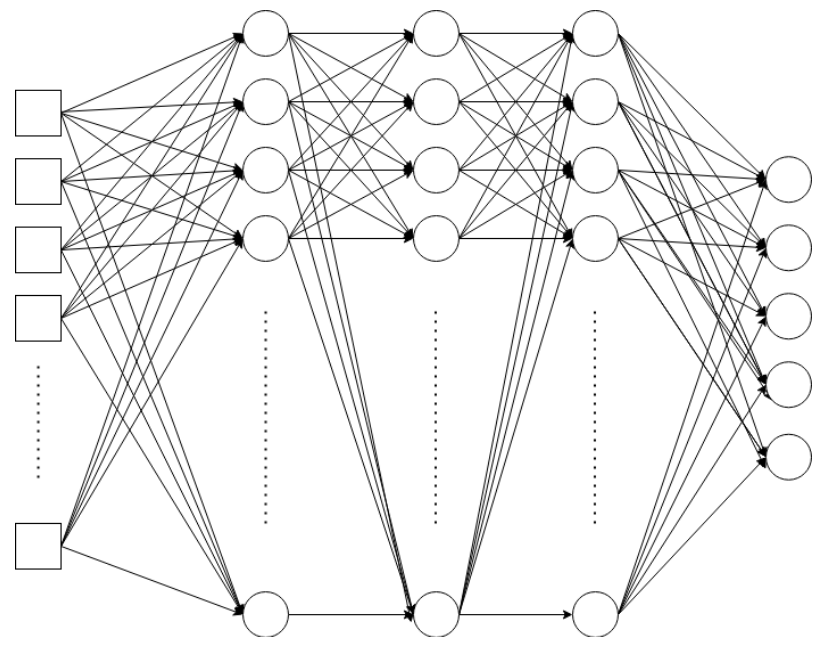
\includegraphics[width=.7\textwidth]{modello}}
    \caption{Modello di rete neurale multistrato.}
    \label{modello}
\end{figure}

Il pacchetto per questa rete neurale è composto da sei moduli, ovvero 1 script e 5 funzioni:

\begin{itemize}
    \item \textbf{Script}:
    \begin{itemize}
        \item \texttt{FiveDigit\_Training}: definisce la procedura di apprendimento per la rete neurale. Genera un file con una matrice dei valori dei pesi calcolati a seguito dell'apprendimento.
    \end{itemize}

    \item \textbf{Funzioni}:
    \begin{itemize}
        \item \texttt{FiveDigit\_DeltaRule}: applica la regola di apprendimento. Viene utilizzata ripetutamente nella fase di training della rete neurale per modificare i valori dei pesi;
        \item \texttt{FiveDigit\_Preparation}: genera una matrice di immagini delle cinque cifre con rumore simulato del tipo ``\emph{salt \& pepper}'';
        \item \texttt{FiveDigit\_Test}: calcola l'errore rispetto all'output corretto tramite una nuova fase di feedforward. Viene applicata in parallelo alla fase di apprendimento: questa fase di test, cioè, viene eseguita ad ogni epoca con i valori aggiornati dei pesi; 
        \item \texttt{ReLU}: funzione di attivazione per i nodi degli strati nascosti;
        \item \texttt{Softmax}: funzione di attivazione per i nodi di output.
    \end{itemize}
\end{itemize}



\newpage
%%%%%%%%%%%%%%%
\section{Codice}

\begin{lstlisting}[style=Matlab-editor,caption=\texttt{FiveDigit\_Training},title=\texttt{FiveDigit\_Training.mat},label=lst:training]
% % Produci un grafico ad ogni run ###
% clear;
% num_run = 5;
% for nu = 1:num_run
% figure;
% hold on;
%
alpha = 0.01;
% alpha = [0.001 0.01 0.05]; %(b1)
% densities = [0.1 0.2]; %(c1)
% num_of_elements_of_test_set = [10 50 100]; %(c2)
num_of_elements_of_training_set = [10 15]; %(c3)
%
for i = alpha % inizio ciclo su alpha
% for k = densities %(c1)
% for j = num_of_elements_of_test_set %(c2)
for l = num_of_elements_of_training_set %(c3)
%   input
%   Immagine della cifra uno
    training_set(:,:,1) = [1 0 0 1 1; 1 1 0 1 1; 1 1 0 1 1; 1 1 0 1 1; 1 0 0 0 1];
%   Immagine della cifra due
    training_set(:,:,2) = [0 0 0 0 1; 1 1 1 1 0; 1 0 0 0 1; 0 1 1 1 1; 0 0 0 0 0];
%   Immagine della cifra tre
    training_set(:,:,3) = [0 0 0 0 1; 1 1 1 1 0; 1 0 0 0 1; 1 1 1 1 0; 0 0 0 0 0];
%   Immagine della cifra quattro
    training_set(:,:,4) = [1 1 1 0 1; 1 1 0 0 1; 1 0 1 0 1; 0 0 0 0 0; 1 1 1 0 1];
%   Immagine della cifra cinque
    training_set(:,:,5) = [0 0 0 0 0; 0 1 1 1 1; 0 0 0 0 1; 1 1 1 1 0; 0 0 0 0 1];
%
%   Output corretti: la cifra 'uni' in colonna 'i' indica che si deve individuare la cifra 'i'
    correct_output = [1 0 0 0 0; 0 1 0 0 0; 0 0 1 0 0; 0 0 0 1 0; 0 0 0 0 1];
%   Inizializzazione casuale dei pesi
    w1 = 2 * rand(20, 25) - 1;
    w2 = 2 * rand(20, 20) - 1; 
    w3 = 2 * rand(20, 20) - 1;
    w4 = 2 * rand(5, 20) - 1;
%
%   Definizione del test set
%     test_set = FiveDigit_Preparation(training_set,20,k); %(c1)
%     test_set = cat(3,training_set,test_set); %(c1)
%     test_set = FiveDigit_Preparation(training_set,j-5,0.1); %(c2)
%     test_set = cat(3,training_set,test_set); %(c2)
    test_set = FiveDigit_Preparation(training_set,45,0.1); %(c3)
    test_set = cat(3,training_set,test_set); %(c3)
%
%   Iperparametro col numero di epoche
    N_epoch = 1000;
%
%   Inizializzazione dei vettori per i grafici
    MSE_Learn = []; % MSE per epoca (apprendimento)
    MSE_Test = [];  % MSE per epoca (test)
    epoch0 = [];    % epoche
%
%   Settaggio di input_image
%    input_image = training_set; %base
%    training_set_noise = FiveDigit_Preparation(training_set,5,0.1); %(b2)
   training_set_noise = FiveDigit_Preparation(training_set,l-5,0.1); %(c3)
   input_image = cat(3,training_set,training_set_noise); %(b2) e (c3)
%
%   Inizia il ciclo di apprendimento sulle epoche
    for epoch = 1:N_epoch
%         correct_output_training_set = correct_output; %base
%         num_di_training_set = 5; %base
%         correct_output_training_set = repmat(correct_output, 2, 1); %(b2) 
%         num_di_training_set = 10; %(b2)
        correct_output_training_set = repmat(correct_output, l/5, 1); %(c3) 
        num_di_training_set = l; %(c3)
        [w1, w2, w3, w4, norDelta, norDelta3, norDelta2, norDelta1, output_matrix] = FiveDigit_DeltaRule(w1, w2, w3, w4, input_image, correct_output_training_set, i, num_di_training_set);
%
%       Concatena l'epoca corrente al vettore delle epoche
        epoch0 = [epoch0 epoch];
%
%       Concatena l'MSE_Learn osservato in fase di  
%       apprendimento sullo strato di output per l'epoca 
%       corrente; calcolato sul training set
        MSE_L = immse(output_matrix, correct_output_training_set);
        MSE_Learn = [MSE_Learn MSE_L];
%
%       Concatena l'MSE_Test osservato dopo l'apprendimento in
%       fase di test; calcolato sul test set
        num_di_test_set = size(test_set,3);
        correct_output_test_set = repmat(correct_output, num_di_test_set/5, 1);
        MSE_T = FiveDigit_Test(w1, w2, w3, w4, test_set, correct_output_test_set, num_di_test_set);
        MSE_Test = [MSE_Test MSE_T];
%
    end % fine ciclo sulle epoche
%
% %   Grafico delle curve di apprendimento con diversi alpha, punti (b1) e (b2)
%     plot(epoch0(1:100),MSE_Learn(1:100),'LineWidth',3), grid;
%     title('Learning Curve (Loss)')
%     xlabel('epoch')
%     ylabel('MSE Learn')
%     legend('alpha 0.001', 'alpha 0.01', 'alpha 0.05');
%     hold on
%
% %   Grafico delle curve loss con diversi test set, punto (c1)
%     plot(epoch0(1:10000),MSE_Test(1:10000),'LineWidth',3), grid;
%     title('Loss Curve con diversi test set')
%     xlabel('epoch')
%     ylabel('MSE Test')
%     leg = legend('dens 0.1', 'dens 0.2');
%     title(leg, 'Test set');
%     hold on
%
% %   Grafico delle curve loss con diversi test set, punto (c2)
%     plot(epoch0(1:1000),MSE_Test(1:1000),'LineWidth',3), grid;
%     title('Loss Curve con diversi test set')
%     xlabel('epoch')
%     ylabel('MSE Test')
%     leg = legend('10 elementi', '50 elementi', '100 elementi');
%     title(leg, 'Test set');
%     hold on
%
%   Grafico delle curve loss con diversi training set, punto (c3)
    plot(epoch0(1:1000),MSE_Test(1:1000),'LineWidth',3), grid;
    title('Loss Curve con diversi training set')
    xlabel('epoch')
    ylabel('MSE Test')
    leg = legend('10 elementi', '15 elementi');
    title(leg, 'Training set');
    hold on
%
% end % ###
% print(strcat('fig-c3-',int2str(nu)),'-depsc') % esporta grafici ###
% hold off; % ###
%
end % (c1) o (c2) o (c3)
end % fine ciclo su alpha
%
% Memorizzazione su file dei valori dei pesi cosi' calcolati
save('FiveDigit_Trained_Network.mat');
\end{lstlisting}


\newpage
\begin{lstlisting}[style=Matlab-editor,title=\texttt{FiveDigit\_DeltaRule.mat}]
function [w1, w2, w3, w4, norDelta, norDelta3, norDelta2, norDelta1, output_matrix] = FiveDigit_DeltaRule(w1, w2, w3, w4, input_image, correct_output, alpha, N)
%
%%%%% Settaggio dei parametri
%
%     alpha = 0.001; % velocita di apprendimento
%     N = 5; %numero delle cifre da apprendere
    output_matrix = zeros(N,5); % matrice Nx5 (immagine) dei valori di output
    reshaped_input_image = zeros(25,1);
%
%%%%% Ciclo sulle cinque cifre
%
    for k = 1:N
%       Ridimensionamento della matrice dell'immagine di 
%       input in un'unica colonna
        reshaped_input_image =reshape(input_image(:,:,k),25,1);
%
%%%%% Inizia la fase di feedforward
%
%       Trasmissione attivazione dallo strato di input a
%       nascosto h1
        input_to_hidden_layer1 = w1*reshaped_input_image;
        output_of_hidden_layer1 = ReLU(input_to_hidden_layer1);
% 
%       Trasmissione attivazione da h1 a h2
        input_to_hidden_layer2 = w2*output_of_hidden_layer1;
        output_of_hidden_layer2 = ReLU(input_to_hidden_layer2);
%
%       Trasmissione attivazione da h2 a h3
        input_to_hidden_layer3 = w3*output_of_hidden_layer2;
        output_of_hidden_layer3 = ReLU(input_to_hidden_layer3);
%
%       Trasmissione attivazione da h3 allo strato di output
        input_to_output_node = w4*output_of_hidden_layer3;
%
%       Normalizzazione dei valori di output tramite Softmax
        final_output = Softmax(input_to_output_node);
%
%       Calcolo della trasposta del correct_output
        correct_output_transpose = correct_output(k, :)';
%
%       Calcolo dell'errore sullo strato di output
        error = correct_output_transpose - final_output;
%
%%%%% Fase di backpropagation
%
%       Calcolo della delta rule
        delta = error;
        norDelta=norm(delta);
%
        error_of_hidden_layer3 = w4'*delta;
        delta3=(input_to_hidden_layer3>0) .* error_of_hidden_layer3;
        norDelta3 =norm(delta3);
%
        error_of_hidden_layer2 = w3'*delta3;
        delta2=(input_to_hidden_layer2>0) .* error_of_hidden_layer2;
        norDelta2 = norm(delta2);
%
        error_of_hidden_layer1 = w2'*delta2;
        delta1=(input_to_hidden_layer1>0) .* error_of_hidden_layer1;
        norDelta1=norm(delta1);
%
%       Calcolo dell'aggiornamento dei pesi tramite delta rule
        update_of_w4 = alpha*delta*output_of_hidden_layer3';
        update_of_w3 = alpha*delta3*output_of_hidden_layer2'; 
        update_of_w2 = alpha*delta2*output_of_hidden_layer1';
        update_of_w1 = alpha*delta1*reshaped_input_image';
%
%       Aggiornamento delle matrici dei pesi
        w1 = w1 + update_of_w1;
        w2 = w2 + update_of_w2;
        w3 = w3 + update_of_w3;
        w4 = w4 + update_of_w4;
%
%       Aggiornamento della matrice degli output
        output_matrix(k,:) = final_output';
%
    end % fine ciclo sulle cifre
end % fine function
\end{lstlisting}


\newpage
\begin{lstlisting}[style=Matlab-editor,title=\texttt{FiveDigit\_Test.mat}]
function MSE_T = FiveDigit_Test (w1, w2, w3, w4, input_image, correct_Output, N)
    learned_Output = zeros([N 5]);
%
    for k = 1:N   % Ciclo sugli stimoli di input
        current_input_image = reshape(input_image(:,:,k),25,1);
%
%       Calcolo dell'output della rete con modalita' feedforward
% 
        input_hidden_1 = w1 * current_input_image;
        output_hidden_1 = ReLU(input_hidden_1);
        input_hidden_2 = w2 * output_hidden_1;
        output_hidden_2 = ReLU(input_hidden_2);
        input_hidden_3 = w3 * output_hidden_2;
        output_hidden_3 = ReLU(input_hidden_3);
        input_output_node = w4 * output_hidden_3;
        final_output = Softmax(input_output_node);
%
%       Memorizzazione dell'output finale nella matrice 
%       learned_Output dopo aver trasposto il final_output
        learned_Output(k,:) = final_output';
%
    end  % fine ciclo sui vettori (stimoli) di ingresso
%
%   Calcolo l'errore MSE_Test tra le due matrici (output della function)
    MSE_T = immse(learned_Output,correct_Output);
%
end  % fine function
\end{lstlisting}


\newpage
\begin{lstlisting}[style=Matlab-editor,caption=\texttt{FiveDigit\_Preparation},title=\texttt{FiveDigit\_Preparation.mat},label=lst:preparation]
function [image] = FiveDigit_Preparation(image, ntest, dens)
    num_ripetizioni = (ntest/5);
    i=1;
    for j=1:num_ripetizioni
        for k=1:5 % numero immagini di input (1,2,3,4,5)
            image(:,:,i) = imnoise(image(:,:,k),'salt & pepper',dens);
            i = i+1;
        end
    end
%
end
\end{lstlisting}


\vspace{1cm}


\begin{lstlisting}[style=Matlab-editor,title=\texttt{ReLU.mat}]
function y = ReLU(x)
    y = max(0,x);
end
\end{lstlisting}


\vspace{1cm}


\begin{lstlisting}[style=Matlab-editor,title=\texttt{Softmax.mat}]
function y = Softmax(x)
    ex = exp(x);
    y = ex/sum(ex);
end
\end{lstlisting}


\newpage
\setcounter{section}{0}
\renewcommand{\thesection}{\alph{section}}
%%%%%%%%%%%%%%%%%%%%%%%%%%%%%%
\section{Preparazione dei dati}

\paragraph{(a1) e (a2)}In \coderef{lst:training} abbiamo definito il training set (righe $18-28$) e il test set (righe $38-44$). Per generare il test set (e i successivi training set) ci siamo serviti della funzione \coderef{lst:preparation}.

\paragraph{(a3)} Abbiamo visualizzato tutte le immagini (originali e rumorose) in Figura~\vref{fig:a3}.

\begin{figure}[htb]
    \centering
    \tcbox[boxrule=.3mm,colback=white]{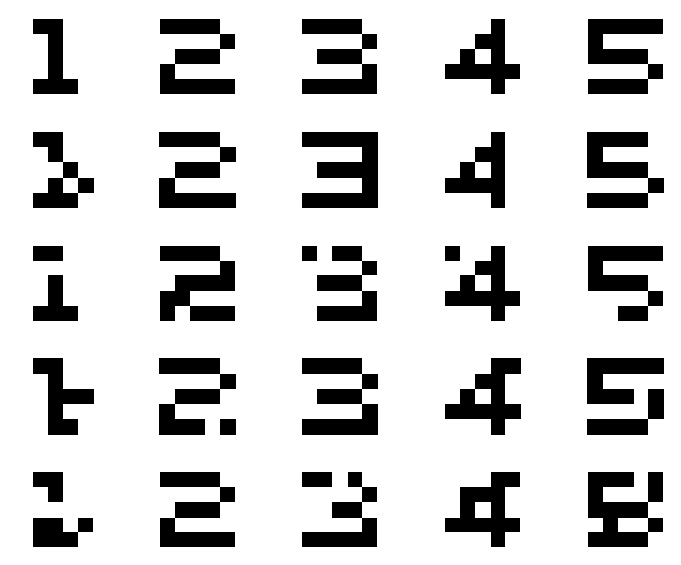
\includegraphics[width=.8\textwidth]{fig-a3.eps}}
    \caption{Immagini originali (prima riga) e rumorose delle cinque cifre.}
    \label{fig:a3}
\end{figure}

Nella prima riga in alto sono riportate le cinque immagini di input, quelle corrette. Le successive quattro righe contengono immagini con errore simulato, ovvero con pixel accesi o spenti dove non dovrebbero esserlo. Questo effetto è stato generato con la funzione Matlab \texttt{imnoise}, in particolare con densità di rumore pari a $0.1$ e con tipo di rumore \emph{salt and pepper}. Questa funzione di aggiunta di rumore ha una componente casuale: è questo il motivo per cui le immagini rumorose sono diverse tra di loro anche a parità di numero (colonna).



\newpage
%%%%%%%%%%%%%%%%%%%%%%%%%%%%%%
\section{Fasi di Apprendimento}

\paragraph{(b1)} Per le cinque immagini originali, abbiamo calcolato le curve di apprendimento al variare del tasso di apprendimento (learning rate) coi valori $alpha=0.001,~0.01,~0.05$. 

L'apprendimento è stato ripetuto per cinque volte, in modo da ottenere cinque grafici (Figg.~\vref{fig:b1-1},~\vref{fig:b1-2} e~\vref{fig:b1-3}). Osservando le immagini, si può notare come il miglior valore di $alpha$ sia $0.01$. Con questo valore, infatti, l'errore raggiunge sempre (a differenza di $alpha=0.05$ che a volte non converge) e più velocemente (a differenza di $alpha=0.001$ che converge più lentamente) la convergenza.

\begin{figure}[htb]
    \centering
    \tcbox[boxrule=.3mm,colback=white]{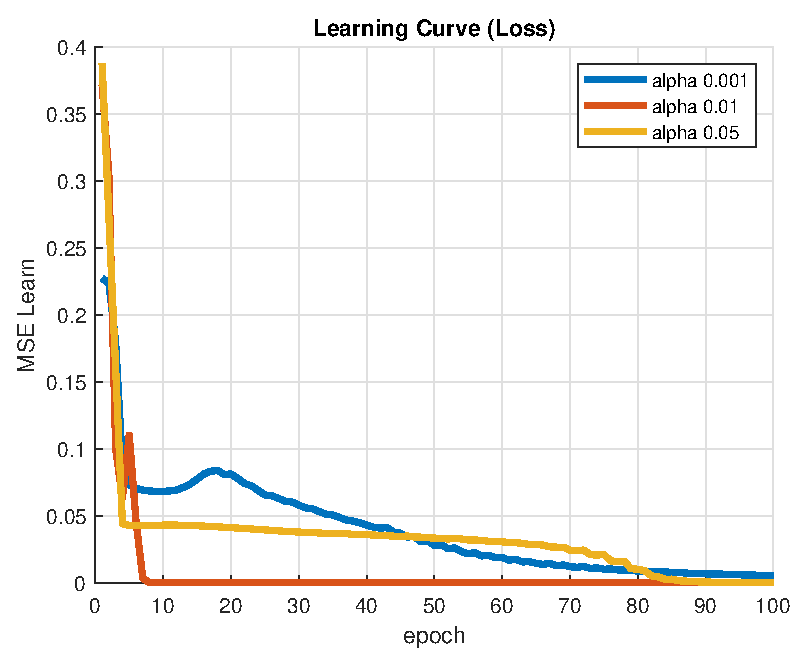
\includegraphics[width=.8\textwidth]{fig-b1-1.eps}}
    \caption{Curve di apprendimento loss al variare di $alpha$ (1/5).}
    \label{fig:b1-1}
\end{figure}

\begin{figure}[htp]
    \centering
    \tcbox[boxrule=.3mm,colback=white]{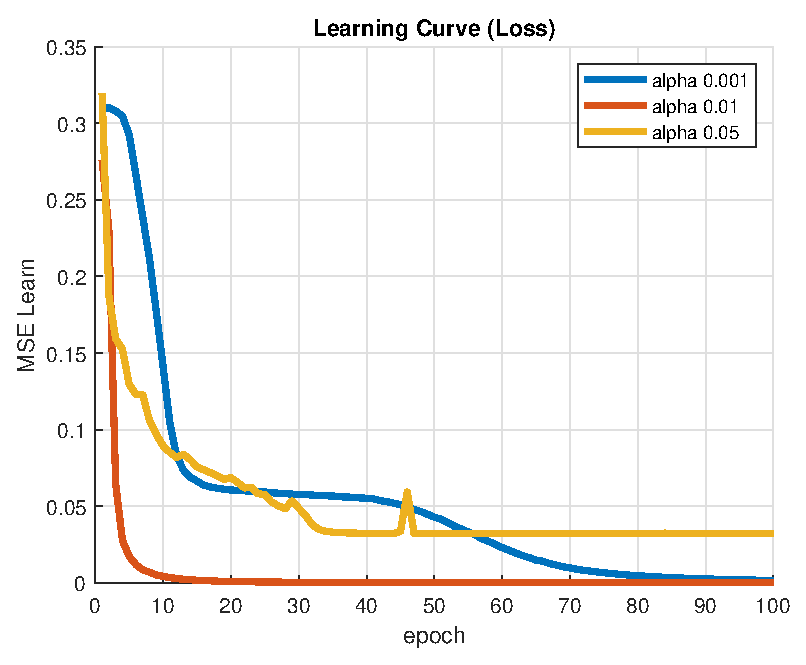
\includegraphics[width=.8\textwidth]{fig-b1-2.eps}}

    \medskip

    \tcbox[boxrule=.3mm,colback=white]{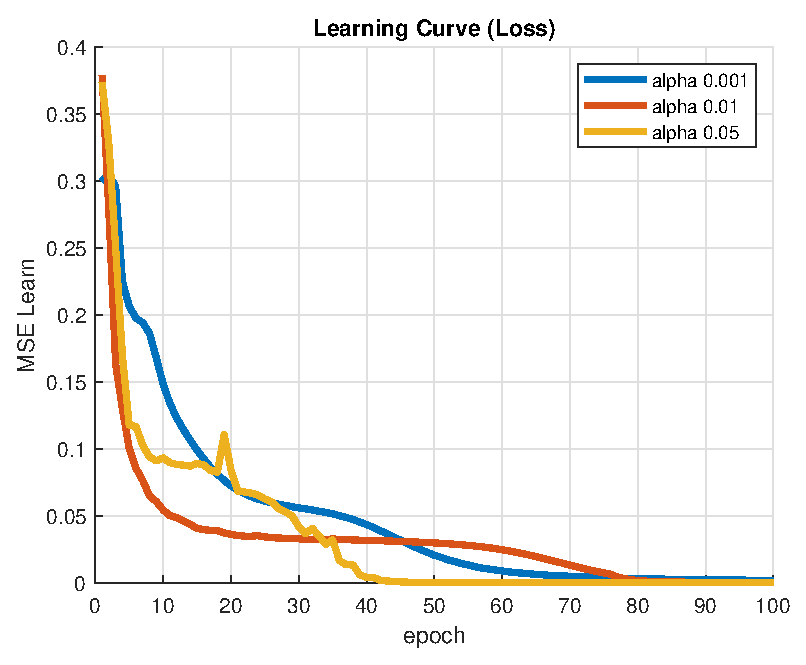
\includegraphics[width=.8\textwidth]{fig-b1-3.eps}}

    \caption{Curve di apprendimento loss al variare di $alpha$ (2/5) e (3/5).}
    \label{fig:b1-2}
\end{figure}

\begin{figure}[htp]
    \centering
    \tcbox[boxrule=.3mm,colback=white]{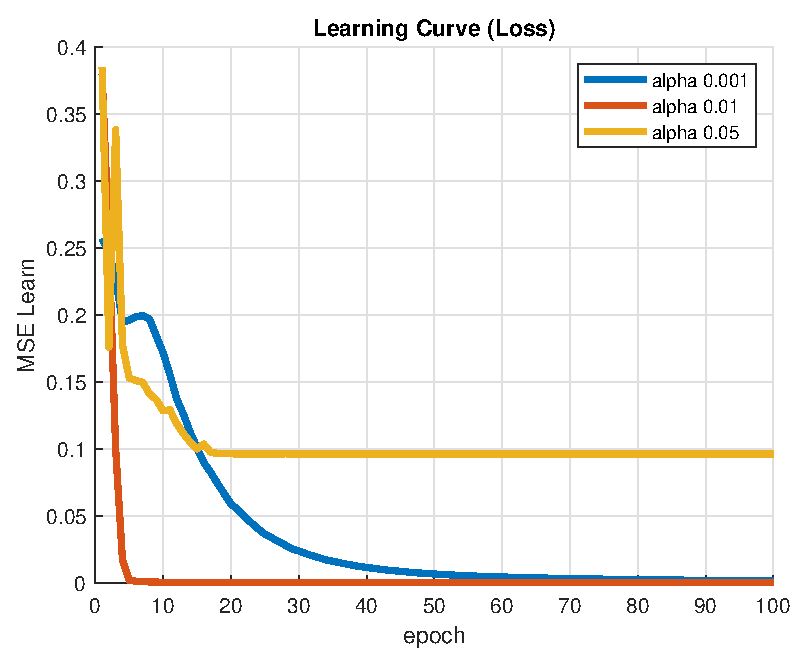
\includegraphics[width=.8\textwidth]{fig-b1-4.eps}}

    \medskip

    \tcbox[boxrule=.3mm,colback=white]{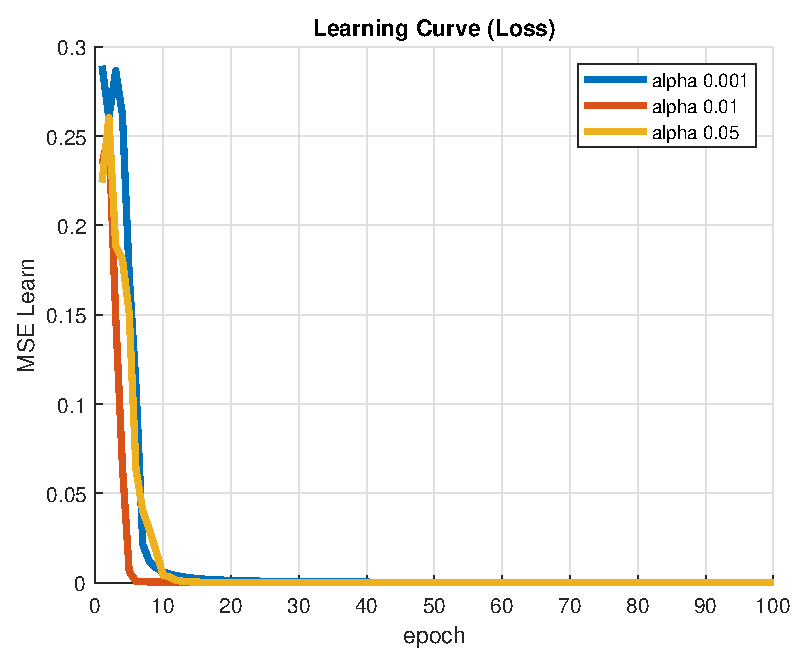
\includegraphics[width=.8\textwidth]{fig-b1-5.eps}}

    \caption{Curve di apprendimento loss al variare di $alpha$ (4/5) e (5/5).}
    \label{fig:b1-3}
\end{figure}


\newpage
\paragraph{(b2)} Abbiamo generato un nuovo training set, aggiungendo alle cinque immagini originali altre cinque immagini rumorose ottenute con $dens=0.1$, una per ogni cifra. Abbiamo quindi ripetuto l'apprendimento con il nuovo training set (Figura~\vref{fig:b2}). 

\begin{figure}[htb]
    \centering
    \tcbox[boxrule=.3mm,colback=white]{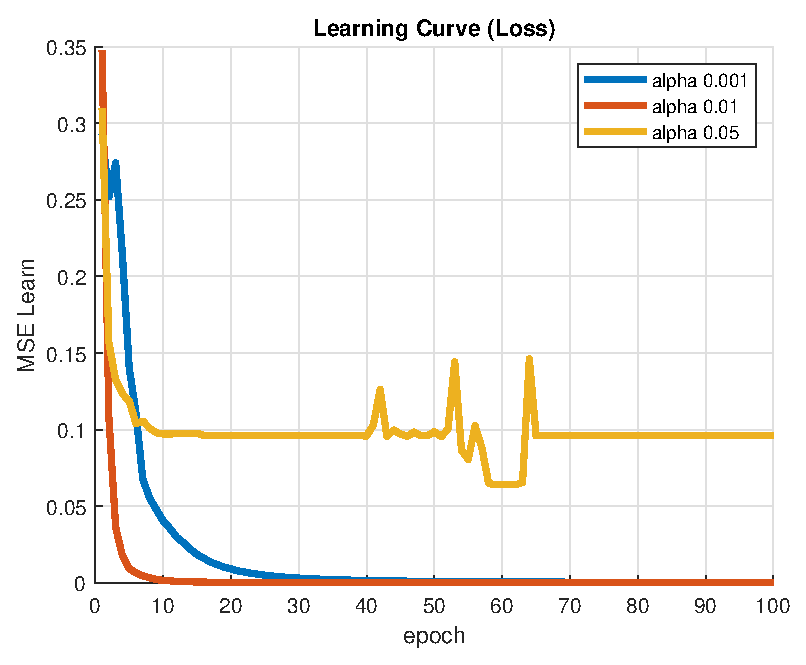
\includegraphics[width=.9\textwidth]{fig-b2-tre-alpha3.eps}}
    \caption{Curve di apprendimento loss al variare di $alpha$, training set con 10 elementi.}
    \label{fig:b2}
\end{figure}

Come si può osservare dal grafico, i risultati sono simili a quelli ottenuti al punto precedente, con un training set costituito dalle sole cinque immagini originali. Anche qui il miglior valore di $alpha$ è $0.01$.



\newpage
%%%%%%%%%%%%%%%%%%%%%%%%%%%%%%
\section{Fasi di Test}

\paragraph{(c1)} Abbiamo generato due distinti test set di $ntest=20$ elementi ciascuno, rispettivamente con densità di rumore $dens=0.1$ e $dens=0.2$. Per ciascuno dei due sono state calcolate le curve loss con $alpha=0.01$.

Sono state effettuate cinque run, i cui grafici sono riportati nelle Figure~\vref{fig:c1-1},~\vref{fig:c1-2} e~\vref{fig:c1-3}. Come si può osservare, l'errore non sempre converge, ma la rete sembra avere delle prestazioni migliori con densità di rumore $0.1$.

\begin{figure}[htb]
    \centering
    \tcbox[boxrule=.3mm,colback=white]{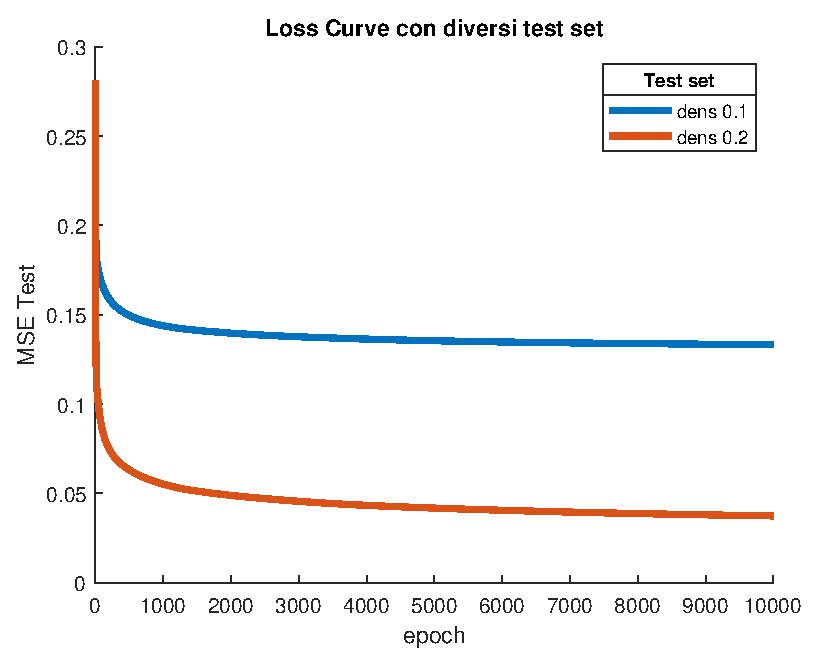
\includegraphics[width=.8\textwidth]{fig-c1-1.eps}}
    \caption{Curve loss (test) relative a due test set con densità di rumore differente (1/5).}
    \label{fig:c1-1}
\end{figure}

\begin{figure}[htp]
    \centering
    \tcbox[boxrule=.3mm,colback=white]{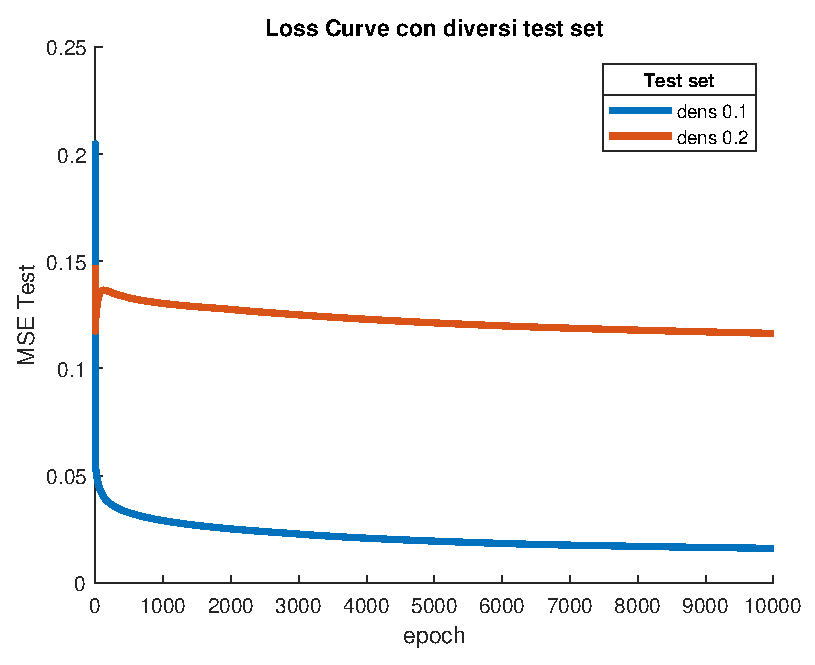
\includegraphics[width=.8\textwidth]{fig-c1-2.eps}}

    \medskip

    \tcbox[boxrule=.3mm,colback=white]{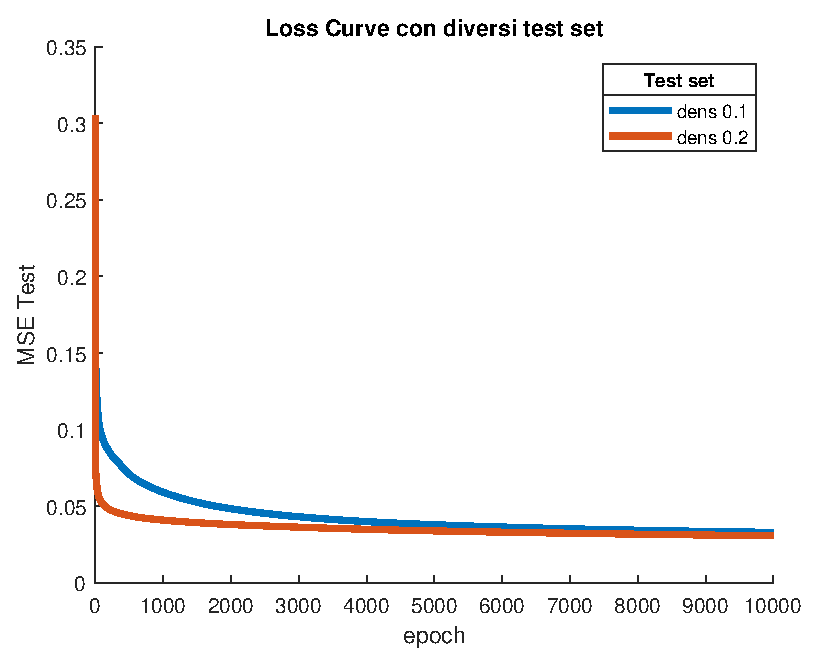
\includegraphics[width=.8\textwidth]{fig-c1-3.eps}}

    \caption{Curve loss (test) relative a due test set con densità di rumore differente (2/5) e (3/5).}
    \label{fig:c1-2}
\end{figure}

\begin{figure}[htp]
    \centering
    \tcbox[boxrule=.3mm,colback=white]{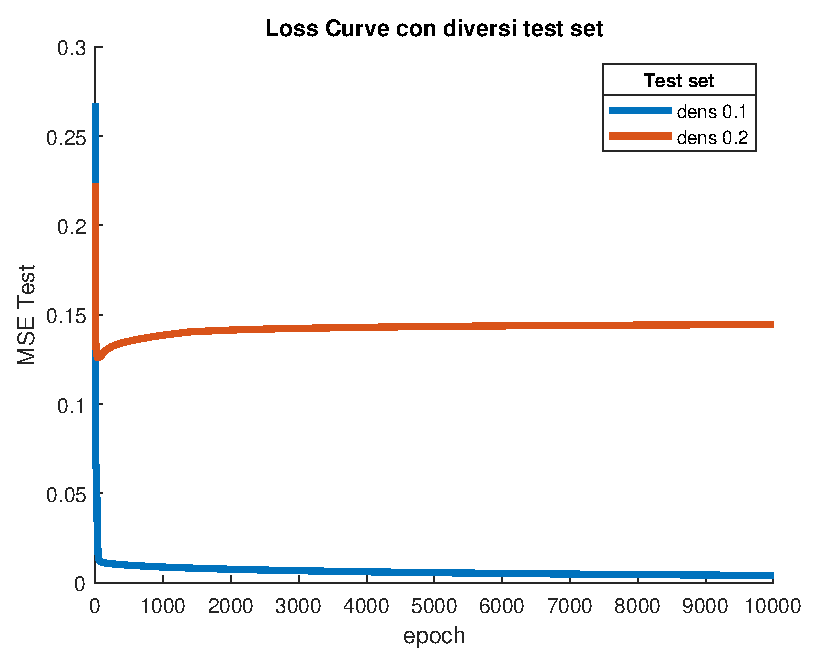
\includegraphics[width=.8\textwidth]{fig-c1-4.eps}}

    \medskip

    \tcbox[boxrule=.3mm,colback=white]{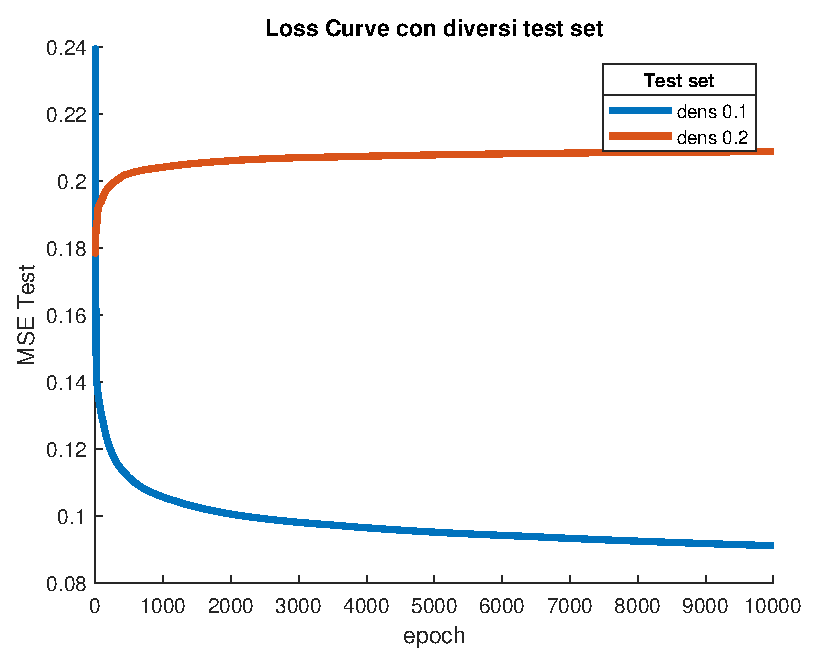
\includegraphics[width=.8\textwidth]{fig-c1-5.eps}}

    \caption{Curve loss (test) relative a due test set con densità di rumore differente (4/5) e (5/5).}
    \label{fig:c1-3}
\end{figure}


\newpage
\paragraph{(c2)} Abbiamo generato tre distinti test set, rispettivamente con $10$, $50$ e $100$ elementi, tutti calcolati con un unico valore $dens=0.1$. Per ciascuno dei test set abbiamo calcolato la curva loss con $alpha=0.01$.

Anche in questo caso sono state effettuate cinque run, i cui grafici sono riportati nelle Figure~\vref{fig:c2-1},~\vref{fig:c2-2} e~\vref{fig:c2-3}. In questo caso l'errore sembra convergere sempre nel caso del test set con $10$ elementi.

\begin{figure}[htb]
    \centering
    \tcbox[boxrule=.3mm,colback=white]{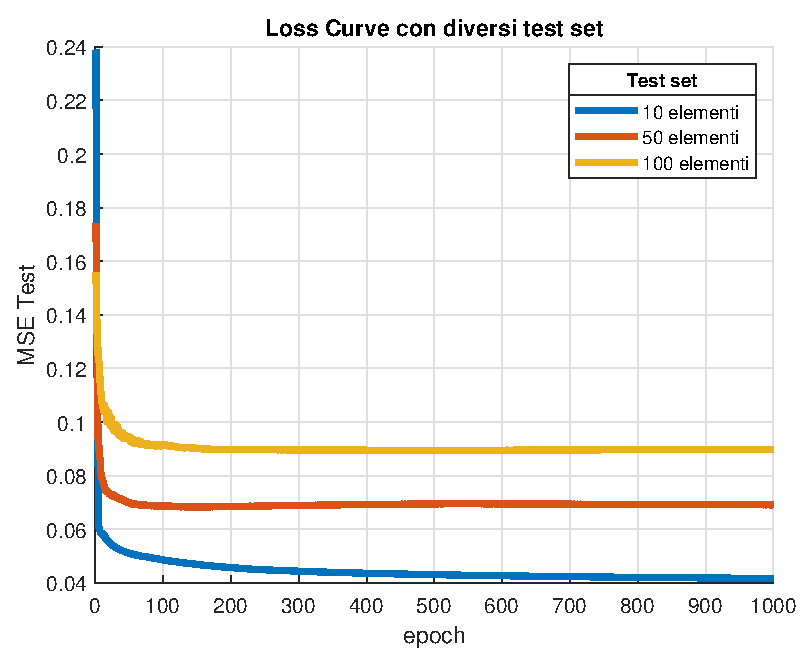
\includegraphics[width=.8\textwidth]{fig-c2-1.eps}}
    \caption{Curve loss (test) relative a tre test set con diverso numero di elementi (1/5).}
    \label{fig:c2-1}
\end{figure}

\begin{figure}[htp]
    \centering
    \tcbox[boxrule=.3mm,colback=white]{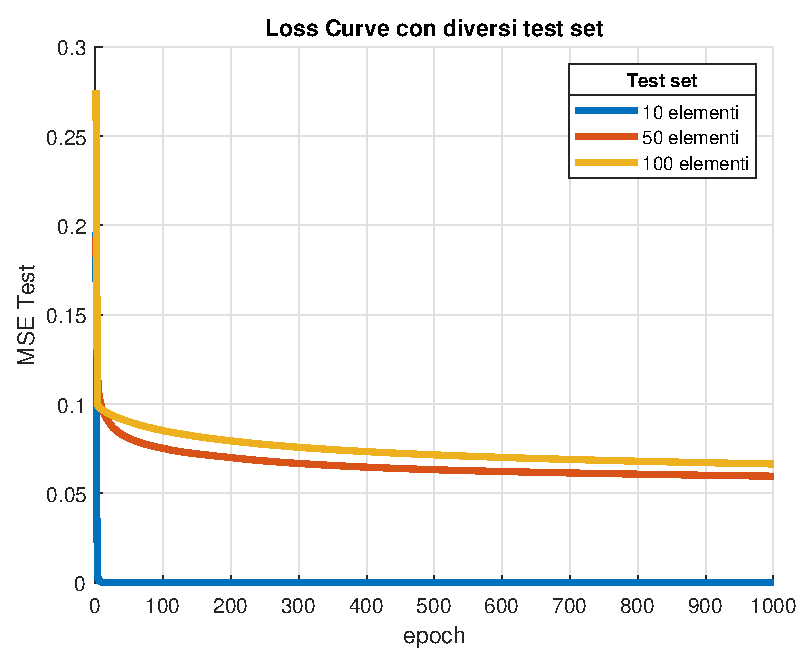
\includegraphics[width=.8\textwidth]{fig-c2-2.eps}}

    \medskip

    \tcbox[boxrule=.3mm,colback=white]{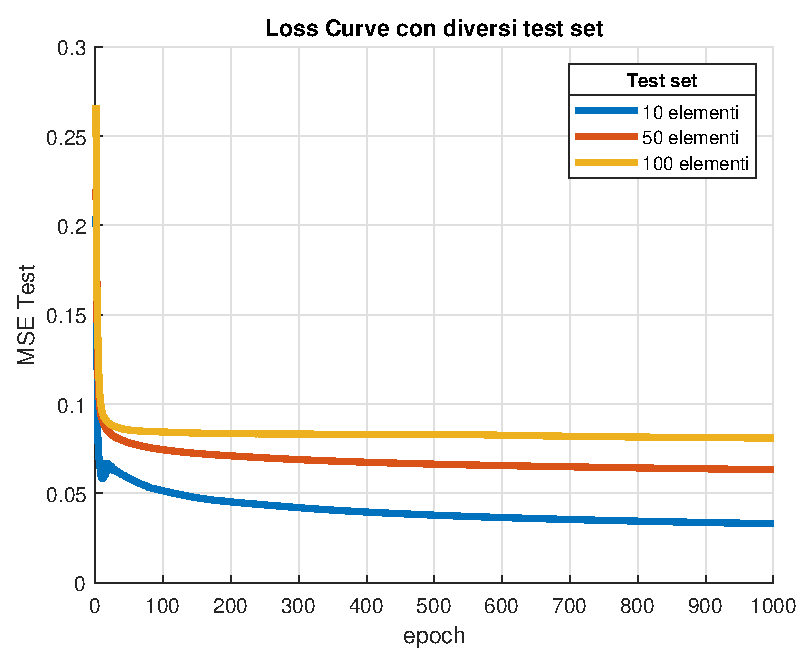
\includegraphics[width=.8\textwidth]{fig-c2-3.eps}}

    \caption{Curve loss (test) relative a tre test set con diverso numero di elementi (2/5) e (3/5).}
    \label{fig:c2-2}
\end{figure}

\begin{figure}[htp]
    \centering
    \tcbox[boxrule=.3mm,colback=white]{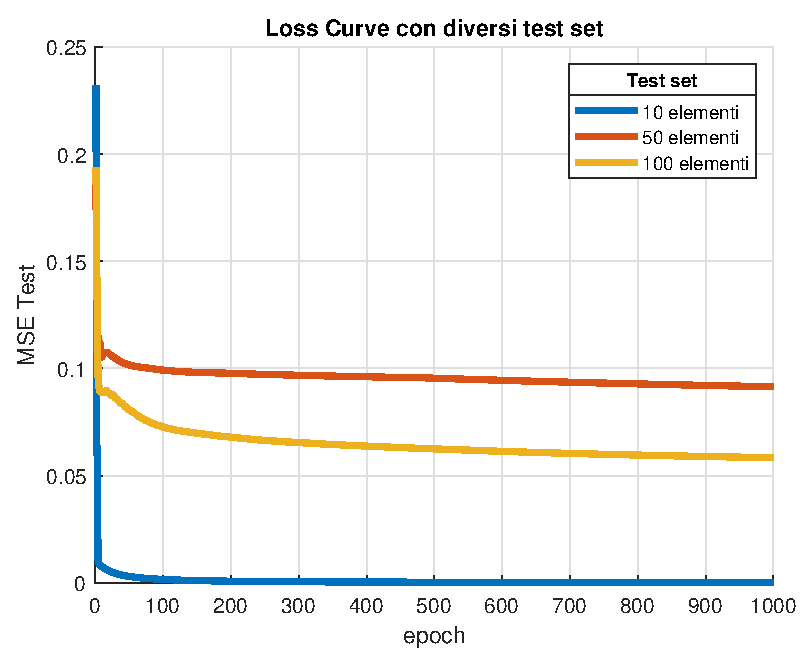
\includegraphics[width=.8\textwidth]{fig-c2-4.eps}}

    \medskip

    \tcbox[boxrule=.3mm,colback=white]{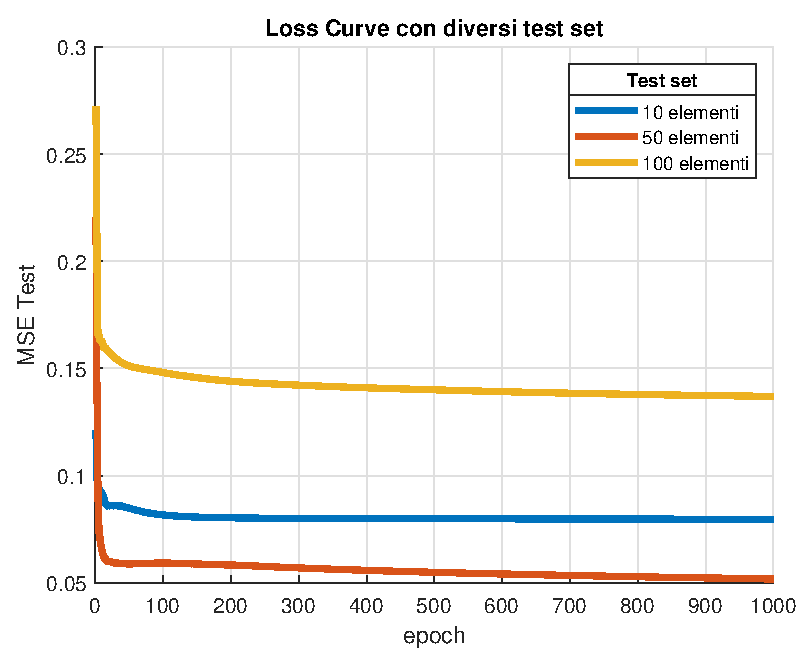
\includegraphics[width=.8\textwidth]{fig-c2-5.eps}}

    \caption{Curve loss (test) relative a tre test set con diverso numero di elementi (4/5) e (5/5).}
    \label{fig:c2-3}
\end{figure}



\newpage
\paragraph{(c3)} Abbiamo esteso il training set con altri $5$, $10$ campioni ricavati dal test set con rumore $dens=0.1$. Per ciascuno dei due casi abbiamo calcolato la curva loss con $alpha=0.01$ rispetto al test set di $50$ elementi.

Sono state effettuate cinque run, i cui grafici sono visibili nelle Figure~\vref{fig:c3-1},~\vref{fig:c3-2} e~\vref{fig:c3-3}. Dalle figure sembrerebbe che l'errore converga sempre e con maggior rapidità nel caso in cui il training set contiene un totale di 15 elementi (5 immagini originali e 10 immagini con rumore).

\begin{figure}[htb]
    \centering
    \tcbox[boxrule=.3mm,colback=white]{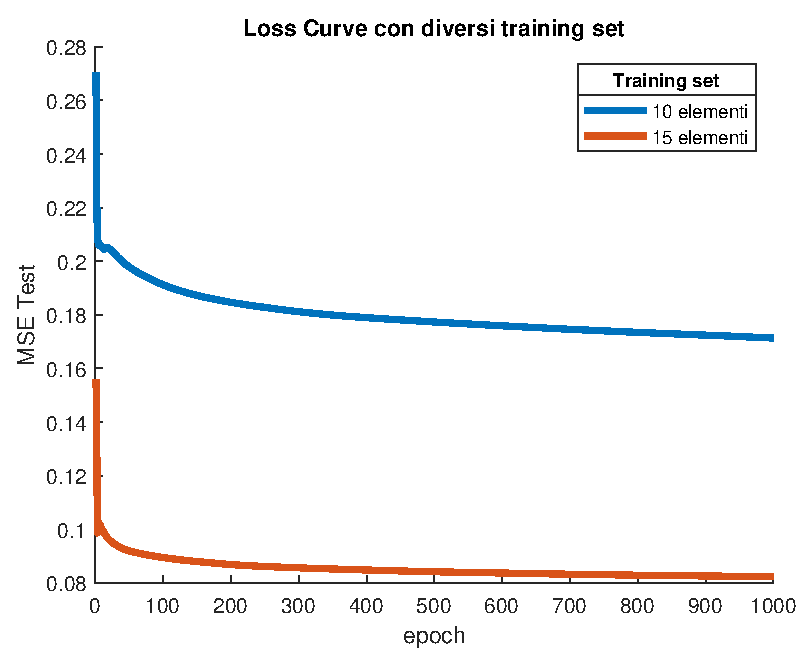
\includegraphics[width=.8\textwidth]{fig-c3-1.eps}}
    \caption{Curve loss (test) relative a due training set con diverso numero di elementi (1/5).}
    \label{fig:c3-1}
\end{figure}

\begin{figure}[htp]
    \centering
    \tcbox[boxrule=.3mm,colback=white]{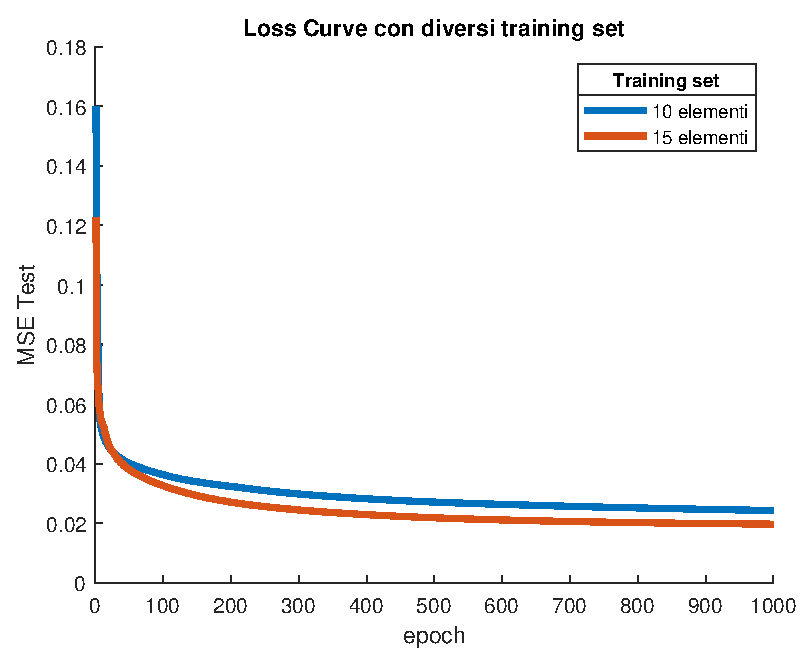
\includegraphics[width=.8\textwidth]{fig-c3-2.eps}}

    \medskip

    \tcbox[boxrule=.3mm,colback=white]{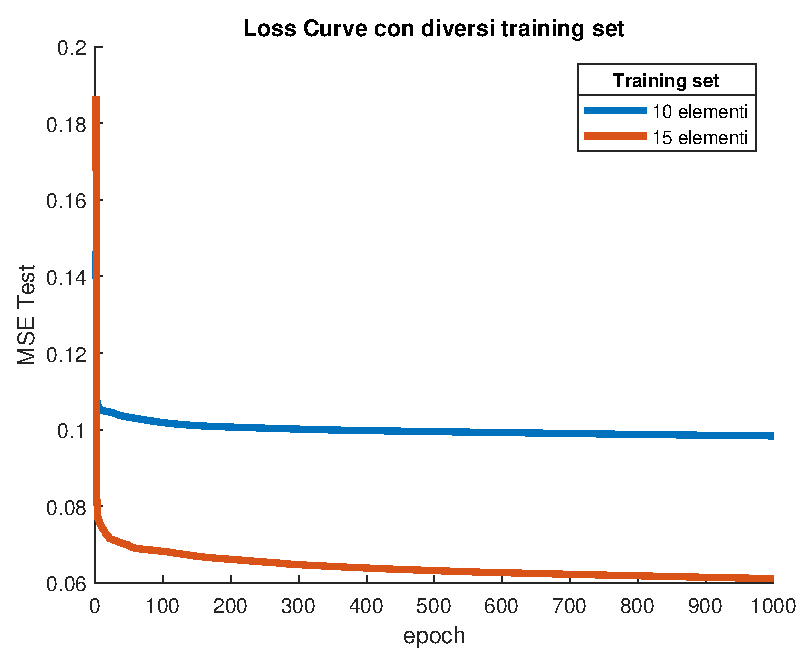
\includegraphics[width=.8\textwidth]{fig-c3-3.eps}}

    \caption{Curve loss (test) relative a due training set con diverso numero di elementi (2/5) e (3/5).}
    \label{fig:c3-2}
\end{figure}

\begin{figure}[htp]
    \centering
    \tcbox[boxrule=.3mm,colback=white]{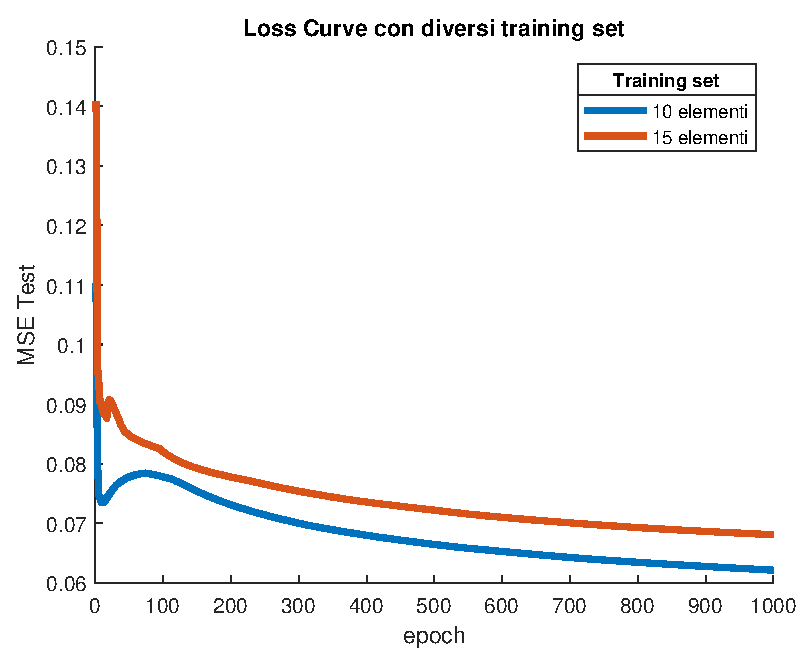
\includegraphics[width=.8\textwidth]{fig-c3-4.eps}}

    \medskip

    \tcbox[boxrule=.3mm,colback=white]{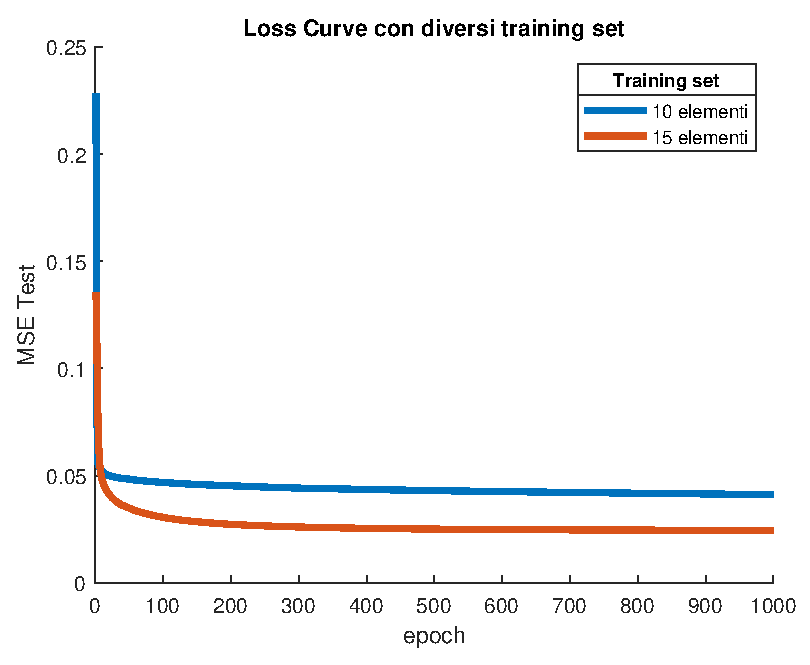
\includegraphics[width=.8\textwidth]{fig-c3-5.eps}}

    \caption{Curve loss (test) relative a due training set con diverso numero di elementi (4/5) e (5/5).}
    \label{fig:c3-3}
\end{figure}



\end{document}